This section will be used to discuss the different attacks on the router and use this to characterize the attacks performed on the honeypot router. The attacks captured on the honeypot will be analyzed in this section to discover the intent of the hackers. This has been done by gathering statistics about the attacks performed on the honeypot by using the methodologies to map the different types of attacks from \textbf{RQ1}. This involves analyzing the different types of attacks performed on the honeypot to discover certain trends or characteristics in the different types of attacks on low-cost routers.

\subsection{General statistics}
The data capture on the honeypot was started on May 17 and the first captured packet was received that day at 12:30 CEST. This data capture lasted until June 4 with the last packet received at 12:45 CEST. After filtering the data capture by removing the IP addresses that could have been originated from the researchers, a total of 1,654,981 packets were remaining. Of these, 872,330 are incoming packets. All packets have a combined size of 184,3MB.

The capture contains a total of 4557 unique IP addresses. The map in Figure \ref{fig:map_attack_location} shows the location of the IP addresses (of which a location was available) and the number of packets received from the location. It can be seen that most of the traffic originated from a small number of source locations.

\begin{figure}[ht]
    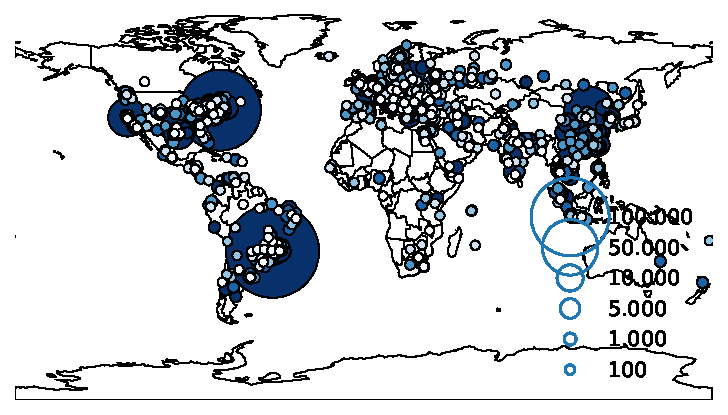
\includegraphics[width=\linewidth]{images/map_attack_locations.pdf}
    \caption{Number of received packets per location}
    \label{fig:map_attack_location}
\end{figure}

The honeypot received traffic from 126 unique countries. Table \ref{table:ip_locations} shows the top countries with incoming traffic. The table also shows the total size of the received packets, the number of unique IP addresses and number of unique Autonomous Systems the IP addresses belong to. As can be seen, the United States of America is the top country with 1.23 times as much traffic originated compared to the number two country, Brazil. When comparing this to the fifth country in terms of received packers, the Republic of Korea, there is almost 12.3 times less traffic compared to the United States of America.

\begin{table}[h]
\centering
\begin{tabular}{ |l|r|r|r|r| } 
\hline
Country & \# packets & size & \# IPs & \# ASNs \\ \hline
US & 230,147 & 22.2MB & 832 & 103 \\ \hline
BR & 186,300 & 17.4MB & 288 & 95 \\ \hline
CN & 115,463 & 12.1MB & 722 & 52 \\ \hline
RU & 19,400 & 1.5MB & 188 & 93 \\ \hline
KR & 18,847 & 1.7MB & 112 & 23 \\ \hline
\end{tabular}
\caption{Top attacker countries}
\label{table:ip_locations}
\end{table}

To understand why the United States, Brazil and China are the largest attacker countries we can take a look at which Autonomous Systems the IP addresses belong to. Traffic was received from a total of 1059 unique Autonomous Systems. Table \ref{table:asn_attacks} displays the top five Autonomous Systems from which most data has been received.

\begin{table}[h]
\centering
\begin{tabular}{ |l|l|r|r|r| } 
\hline
ASN & owner & \# packets & size & \# IPs \\ \hline
AS14061 & DigitalOcean & 175,820 & 17.4MB & 502 \\ \hline
AS8075 & Microsoft & 145,377 & 14.4MB & 16 \\ \hline
AS15169 & Google & 49,121 & 4,8MB & 150 \\ \hline
AS45090 & Tencent & 29,801 & 2.9MB & 42 \\ \hline
AS4134 & Chinanet & 29,422 & 3.6MB & 269 \\ \hline
\end{tabular}
\caption{Top attacker Autonomous Systems}
\label{table:asn_attacks}
\end{table}

Most of the largest subnets traffic has been received from are owned by large cloud providers from China, the United States of America and Brazil. This could also explain the large number of traffic received from these countries as cloud providers can offer capacity, affordability and flexibility. These systems are a common source for attacks as criminals often avoid paying for these systems by taking advantage of free services and trials or by hacking legitimate accounts for their attacks according to research by Akamai, an American Content Delivery Network (CDN) \cite{DDOSCSP:AKAMAI:2019}. This could be an explanation for the large number of traffic from these countries. As a sidenote, 97\% of the traffic from the Autonomous System from Microsoft originated from a single host.

To get a better understanding of when traffic was received and where the traffic originated from, the graph in Figure \ref{fig:data_time_continent} was created to display the amount of received data per continent for each period of 12 hours. This clearly shows a peak a few hours after creation of the honeypot, which displays the moment when the honeypot was discovered by automated systems from attackers. The hackers discover the open services at the IP, attempt to break into the router and after many unsuccessful attempts continue with other devices. The largest attacker at the first peak comes from the DigitalOcean Autonomous System. Another peak is at May 29, when one large large brute-force attacks was attempted from servers of Microsoft Azure in Brazil.

\begin{figure}[ht]
    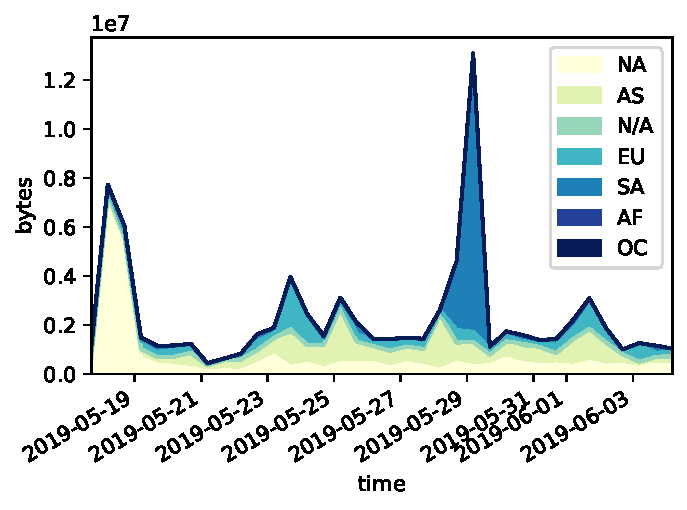
\includegraphics[width=\linewidth]{images/data_time_continent.pdf}
    \caption{Traffic received per continent for each 12 hour time period}
    \label{fig:data_time_continent}
\end{figure}

The top IP address has sent a total of 141,234 packets and 13.9MB of data and orginated from a Brazilian attacker from the Microsoft Azure ASN. The only other sending a similar amount of traffic is an attacker from the DigitalOcean ASN, which sent a total of 11.2MB. As displayed in Figure \ref{fig:ip_packet_cdf}, the number of packets per IP quickly declines, and more than half of the IP addresses never sent more than ten packets. Half of the data has been sent by only 55 IP addresses, which is 1.21\% of the total number of IP addresses. The top IP address has sent 23\% of the packets. The number of IP addresses in the graph has been displayed on a logarithmic scale for readability. 

\begin{figure}[ht]
    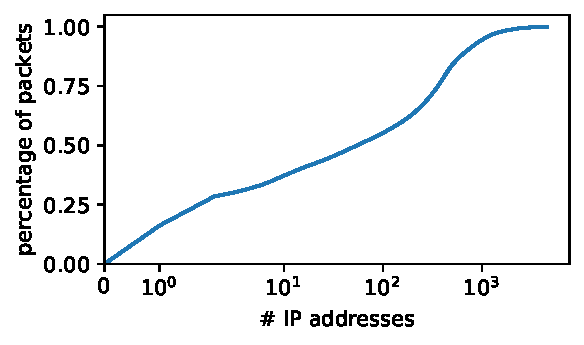
\includegraphics[width=\linewidth]{images/ip_packet_cdf.pdf}
    \caption{CDF of packets and IP addresses}
    \label{fig:ip_packet_cdf}
\end{figure}

Figure \ref{fig:dest_port_graph} shows the distribution of destination ports. Most traffic was targeted at the SSH server at port 22 and the Telnet server at port 23. Much less traffic was received at the web interface at port 80 and the WinBox port 8291. Almost no traffic was received on the SMB service on port 139, the MikroTik-bandwidth-test-server on port 2000 and the FTP server on port 21.

The SSH and Telnet server mostly received multiple large untargeted brute-force attacks trying many standard username and password combinations. Automating brute-force attacks for a common service such as SSH or Telnet is easier than targeting web interfaces on port 80 that differ between manufacturer and model. For this research the traffic on port 8291 is most relevant as this port is used to run the WinBox service and vulnerability CVE-2018-14847 is applicable to this port, therefore increasing the chance of receiving targeted attacks on this port. The low number of packets on port 139 could be an indicator that CVE-2018-7445 is not commonly exploited by attackers.

\begin{figure}[ht]
    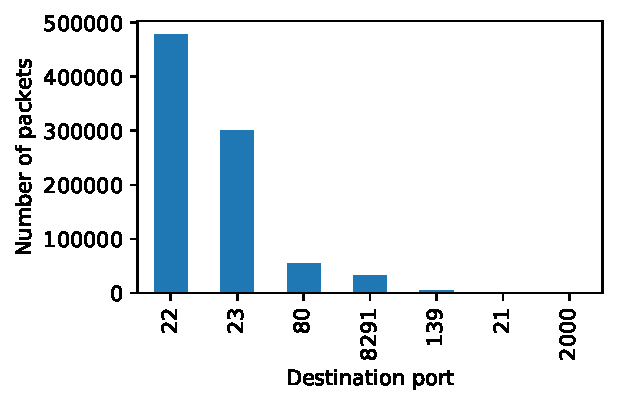
\includegraphics[width=\linewidth]{images/dest_port_packet_graph.pdf}
    \caption{Number of received packets per destination port}
    \label{fig:dest_port_graph}
\end{figure}

There is no clear pattern in the distribution of source ports, as the ports numbers are distributed evenly and the only 282 packets have been received from the top source port. Traffic has been received from a total of 32,788 unique source ports amounting to an average of only 27 received packets per source port.

\subsection{CVE-2018-14847}
The honeypot received large amounts of traffic targeting the critical vulnerability CVE-2018-14847. By filtering the traffic on the TCP streams containing containing one of the payloads, we discovered a total of 3,361 unique TCP streams, which combined amounts to 2.3\% of all in and outgoing traffic on the honeypot, which is quite a significant number considering most traffic is related to simple brute force attacks on the SSH and Telnet ports and that this vulnerability only applies to MikroTik devices. Comparing this to all traffic on port 8291, we can see that this is 71.1\% of all traffic on this port is related to CVE-2018-14847. All attacks targeting this vulnerability exploited this vulnerability to acquire the credentials of the administrator account, while none of the attackers used this vulnerability to enable a root shell on the router or for other purposes.

Around the same time period, other security researchers from GreyNoise Intelligence discovered a 6,700\% increase in attack and scan traffic on port 8291 targeting this vulnerability on their honeypots \cite{6700INC14847:TWITTER:2019}. This was discovered at June 12, eight days after the data capture for this research was halted. To discover if the data of this research supports a similar pattern a graph was made with traffic related to CVE-2018-14847 and the time, which is displayed in Figure \ref{fig:CVE-2018-14847-TRAFFIC}.

\begin{figure}[ht]
    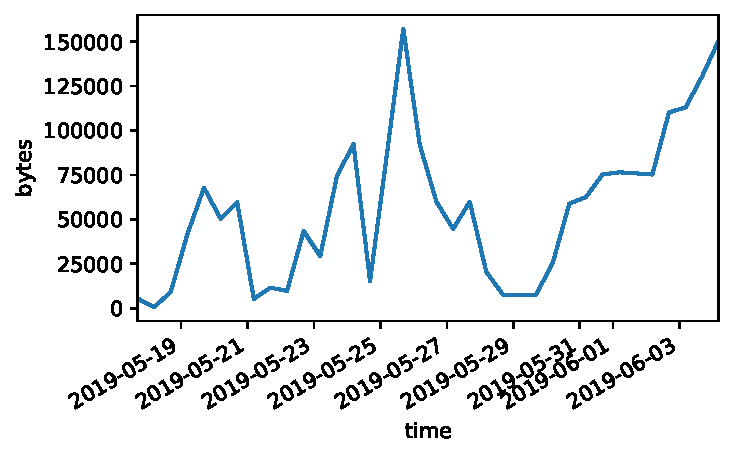
\includegraphics[width=\linewidth]{images/cve_14847_traffic.pdf}
    \caption{Traffic related to CVE-2018-14847 for each 12 hour time period}
    \label{fig:CVE-2018-14847-TRAFFIC}
\end{figure}

A spike in traffic related to CVE-2018-14847 can be seen around May 26 after which the traffic declines and after May 31 the traffic increases to approximately the same amount of traffic as the first spike. The biggest increase in traffic experienced is between the period of May 31 to June 4, which is an increase of 1,974\%. This increase is not close to the 6,700\% discovered by GreyNoise Intelligence. The increase was discovered eight days after the data capture for this research was finished. Therefore, this research does not have enough data to confirm or deny their statement. 

Table \ref{table:asn-cve-14847} shows the autonomous systems related to the attacks on CVE-2018-14847. Traffic was received from a total of 111 unique IP addresses and five Autonomous Systems. The top Autonomous System is the Google Cloud Platform (GCP) with attacks from 106 unique IP addresses originating there.

\begin{table}[h]
\centering
\begin{tabular}{ |l|l|r|r|r| } 
\hline
ASN & owner & \# packets & size & \# IPs \\ \hline
AS15169 & Google & 22,353 & 2.0MB & 106 \\ \hline
AS205544 & Leaseweb & 54 & 4.8KB & 2 \\ \hline
AS51167 & Cantabo & 14 & 1.2KB & 1 \\ \hline
AS42387 & Svyazservice & 8 & 641b & 1 \\ \hline
AS62403 & Disk Group & 7 & 637b & 1 \\ \hline
\end{tabular}
\caption{CVE-2018-14847 Autonomous Systems}
\label{table:asn-cve-14847}
\end{table}

The Google Autonomous System includes the BGP ranges belonging to the Google Cloud Platform. To understand why nearly all attackers for CVE-2018-14847 chose to use the Google Cloud Platform, we decided to examine the offerings of the Google Cloud Platform. As research by the security company Akamai showed, criminals often avoid paying by either taking advantage of free trials or by hijacking legitimate accounts. For this reason, we decided to look if the Google Cloud Platform offers free trials or service or if it is more competitive than either Microsoft Azure or Amazon Web Services.

The Google Cloud Platform offers one basic virtual machine per month\footnote{See: \url{https://cloud.google.com/free/} (18 June 2019)} with no time limit. The competitor, Amazon Web Services has a free tier with a free virtual machine with a 750 hour limit\footnote{See: \url{https://aws.amazon.com/free} (19 June 2019)} and Microsoft Azure offers a similar free virtual machine with a 750 hour limit \footnote{See: \url{https://azure.microsoft.com/free/} (19 June 2019)}. Furthermore, the Google Cloud Platform offers a free Google Cloud Shell to anyone owning a Google account, providing attackers access to a complete Linux virtual machine accessible from a web browser with root capabilities and few limitations\footnote{See: \url{https://cloud.google.com/shell/} (18 June 2019)}. For this type of attack, it could be that Google Cloud Platform is more popular by attackers than the free services of the competitors, because it provides the free virtual machines and the Cloud Shell.

\subsection{DNS redirection}
The honeypot experienced a significant number of DNS redirection attempts. All of these attempts were received on port 80 and 8291. Of this traffic, 55.3\% of these on port 80 and the other 44.7\% on port 8291. Most of these attempts originated from the same hosts as the attacks targeting CVE-2018-14847. At least some of these attacks were successful, as some attackers succeeded in updating the DNS servers on the router to servers hosted in the Google Cloud Plaform. The attackers exploited the CVE-2018-14847 vulnerability to acquire the user database. This database was then decrypted to retrieve the credentials of the administrator account and the attacker continued by signing in to the router management interface to update the DNS settings.

The traffic related to DNS redirection attacks is 1.5\% of the traffic, excluding the 2.3\% related to CVE-2018-14847. By splitting this up per port we can see that 21.0\% of all traffic on port 8291 is related to DNS redirection attacks and 23.3\% of all traffic on port 80. Of the 2.3\% five different types of untargeted attacks were discovered, targeting D-Link, ARG, DSLink, Secutech and TOTOLINK routers \cite{DLINK:DNSHIJACK:2019}. Table \ref{table:dns_redirection_requests} shows the different brands with the number of observed requests and the request itself.

\begin{table}[h]
\centering
\begin{tabular}{ |l|l|l| } 
\hline
Brand & count & DNS redirection request \\ \hline
ARG & 393 & /form2dns.cgi?dnsmode=1?...\\ \hline
D-Link & 785 & /dnscfg.cgi?dnsPrimary=...\\ \hline
DSLINK & 393 & /action?dns\_status=1...\\ \hline
Secutech & 785 & /wan\_dns.asp?go=...\\ \hline
TOTOLINK & 393 & /boafrm/formbasesetcpipsetup.. \\ \hline
\end{tabular}
\caption{Number of DNS redirection attacks per router brand}
\label{table:dns_redirection_requests}
\end{table}

All requests were observed at least 393 times, with only the TOTOLINK and Secutech being targeted almost twice. By digging further in the traffic we observed a pattern where in each attack, except for one, an attacker sent one request for the TOTOLINK, DSLINK and ARG routers and two requests for the Secutech and D-Link routers. The attacks on port 8291 were usually followed by traffic related to CVE-2018-14847 from the same hosts. This specific characteristic is an indicator that the DNS redirection attacks and the attacks exploiting CVE-2018-14847 could be coming from one or a small group of attackers. Another argument pointing in this direction is that all of the 82 IP addresses performing this attack and nearly all of the traffic related to CVE-2018-14847 originates from the Google Cloud Platform and there is a large overlap in IP addresses related to the DNS redirection attacks and the CVE-2018-14847 vulnerability.

By looking at the IP addresses of the DNS servers included in the requests, five different waves of attacks were discovered, each with a different rogue DNS server. The first of these rogue DNS servers was hosted in Microsoft Azure and the other four were hosted in the Google Cloud Platform. These five DNS servers filtered the incoming DNS requests, making it difficult to discover the intent of the attackers.

\subsection{Point-to-Point Tunneling Protocol}
Another attack that was discovered on the honeypot is a single attack by an attacker from Palestine. The attacker managed to sign in to the system via the WinBox program on port 8291. The logging entries in Table \ref{table:pptp_attack_log} show that the attacker signed in via the WinBox program to change the Point-to-Point Tunneling Protocol (PPTP) settings with the intent of setting up a tunneled connection to the outside. This is a targeted attack, since the user accounts have a strong password and no successful brute-force attempt has been discovered. There is no other traffic from this Palestinian IP, so it cannot be confirmed what method was used by the attacker to acquire the administrator credentials. CVE-2018-14847 is the most likely vulnerability, as this vulnerability has been confirmed to be used by other attackers to retrieve the administrator credentials.

\begin{table}[h]
\centering
\begin{tabular}{ |l|l| } 
\hline
time & message \\ \hline
01:49:59 & user admin logged in from <ip> via winbox \\ \hline
01:50:07 & PPTP Server settings changed by admin \\ \hline
01:50:52 & ppp profile <default> changed by admin \\ \hline
01:51:08 & ppp secret <ppp1> added by admin \\ \hline
01:51:09 & user admin logged out from <ip> via winbox \\ \hline
\end{tabular}
\caption{Log messages for the PPTP attack}
\label{table:pptp_attack_log}
\end{table}

\subsection{IoT Malware}
The honeypot did receive a lot of traffic related to IoT Malware. The total traffic was filtered to discover if there is any traffic related to the Mirai malware, as there is a filter available to detect traffic related to Mirai \cite{IMPROVINGIOTBOTNET:SENSORS:2018}. From this we discovered that a total of 1.0\% of the traffic is related to Mirai, which is a total of 8091 incoming and outgoing packets. Of the traffic, 95.4\% was targeted at the Telnet server on port 23, 4.1\% targeted the SSH server at port 22 and 0.5\% targeted the web service at port 80.

All traffic related to Mirai can be characterized by connecting and after an ACK packet has been received resetting the connection by sending a packet with the RST flag. Of the Mirai traffic, 19.5\% of the packets are RST packets. The server receiving the packet usually then responds with TCP Retransmission packets, which is 41.8\% of the Mirai related packets. There were a total of unique 2212 IP addresses, which is 48.5\% of all the IP addresses.

Most of the vulnerable devices can be attributed to three Chinese Autonomous System: Hi-Net, Chinanet and the CNCGroup, which combined have 25.3\% of all the infected devices from which traffic has been received. Other large Autonomous Systems include TE-AS from Egypt, Rostelecom from Russia and IBSNAZ from Italy. The first infected cloud provider is Digital Ocean with 168 infected IP addresses. Mirai mostly targets vulnerable Internet of Things devices, such as IP cameras \cite{UNDERSTANDINGMIRAI:USENIX:2017} and for this reason most of the Mirai related traffic has been received from local Internet Service Providers (ISPs) and not from cloud services.

\subsection{Denial-of-Service}
During the phase of data capture with the honeypot, we discovered that the honeypot sometimes rebooted multiple times per day and in some cases a few times per hour. By looking at the logs, many of these reboots could be confirmed, but not all of them. This is because the logs only capture the current information every five minutes and the logs were not able to be retrieved every time. After May 20 on 22:15 CEST no log data is available. This is after an attacker entered the system and changed the DNS and the PPTP settings to an IP address of one of the rogue DNS servers from the DNS redirection attempts. After the attack the router closed off all incoming TCP connections by responding with a FIN packet. This stopped on May 22 14:40 CEST when the DNS server was discovered and removed from the DNS settings. Since then the traffic continued like normal. Due to this attack the live diagnostics script was unable to retrieve any log file from the router during that period.

A total of 71 reboots could be confirmed from the logs. When the router reboots, the logs are cleared and a log entry is added showing the time of reboot. As mentioned before, the number of reboots is estimated to be higher as no data is available for May 21 and the logs are only captured every five minutes. The last observed reboot was at May 23 at 15:34 CEST. Just after that time, we updated the Simple Network Management Protocol (SNMP) configuration and enabled Universal Plug and Play (UPnP). After these changes, no reboot has been observed. In Figure \ref{fig:observered_reboots} the number of confirmed reboots is displayed for the period between May 17 and May 25.

\begin{figure}[ht]
    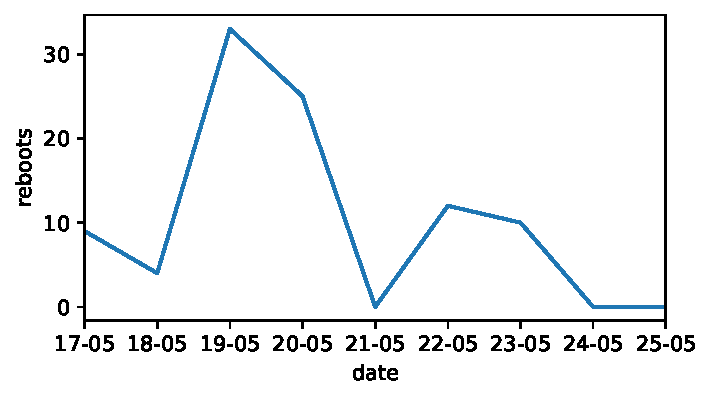
\includegraphics[width=\linewidth]{images/reboots_plot.pdf}
    \caption{Number of confirmed reboots per day}
    \label{fig:observered_reboots}
\end{figure}

To get a better understanding of the cause of the reboots, the logs were compared with the network traffic. Most of the time, the reboot occured after one or multiple RST packet was received from a device infected with the Mirai malware. This is similar to CVE-2017-7285, as in this vulnerability the router is prevented the router from establishing new TCP connections after a flood of RST packets is received \cite{CVE-2017-7285:CXSECURIITY:2017}. The main difference between this attack and CVE-2017-7285 is that CVE-2017-7285 is not confirmed to cause reboots and CVE-201707285 has already been patched in the release of RouterOS used in the honeypot. For these reasons it is unlikely that these reboots are caused by CVE-2017-7285, although a similar vulnerability might be the cause of the observed reboots.